\documentclass{article}

\usepackage{graphicx}
\usepackage{rotating}
\usepackage{amsmath}
\usepackage{fancyhdr}
\usepackage{listings}
\usepackage{xcolor}
\usepackage{color}
\usepackage{textcomp}
\usepackage{float}
\usepackage{titlesec}
\usepackage[sorting=none]{biblatex}
\usepackage[margin=1in]{geometry}
\usepackage[font={small,it}]{caption}
\usepackage{placeins}
\usepackage{xepersian}

%\DeclareMathOperator*{\btie}{\bowtie}
\addbibresource{bibliography.bib}
\settextfont[Scale=1.2]{B-NAZANIN.TTF}
\setlatintextfont[Scale=1]{Times New Roman}
\renewcommand{\baselinestretch}{1.5}
\pagestyle{fancy}
\fancyhf{}
\rhead{پروژه‌ی دوم درس شبکه‌های کامپیوتری 2}
\lhead{\thepage}
\rfoot{علیرضا ابره فروش}
\lfoot{9816603}
\renewcommand{\headrulewidth}{1pt}
\renewcommand{\footrulewidth}{1pt}
%%%%%%%%%%
\lstset
{
    language=[latex]tex,
    basicstyle=\ttfamily,
    commentstyle=\color{black},
    columns=fullflexible,
    keepspaces=true,
    upquote=true,
    showstringspaces=false,
    morestring=[s]\\\%,
    stringstyle=\color{black},
}
%%%%%%%%%%
%beginMatlab
\definecolor{mygreen}{RGB}{28,172,0} % color values Red, Green, Blue
\definecolor{mylilas}{RGB}{170,55,241}
%endMatlab
\begin{document}
%beginMatlab
\lstset{language=Matlab,%
    %basicstyle=\color{red},
    breaklines=true,%
    morekeywords={matlab2tikz},
    keywordstyle=\color{blue},%
    morekeywords=[2]{1}, keywordstyle=[2]{\color{black}},
    identifierstyle=\color{black},%
    stringstyle=\color{mylilas},
    commentstyle=\color{mygreen},%
    showstringspaces=false,%without this there will be a symbol in the places where there is a space
    numbers=left,%
    numberstyle={\tiny \color{black}},% size of the numbers
    numbersep=9pt, % this defines how far the numbers are from the text
    emph=[1]{for,end,break},emphstyle=[1]\color{red}, %some words to emphasise
    %emph=[2]{word1,word2}, emphstyle=[2]{style},    
}
%endMatlab
\begin{titlepage}
\begin{center}

\includegraphics[width=0.4\textwidth]{figures/IUT Logo.png}\\
        
\LARGE
\textbf{دانشگاه صنعتی اصفهان}\\
\textbf{دانشکده مهندسی برق و کامپیوتر}\\
        
\vfill
        
\huge
\textbf{عنوان: تکلیف چهارم درس ریزپردازنده}\\
        
\vfill
        
\LARGE
\textbf{نام و نام خانوادگی: علیرضا ابره فروش}\\
\textbf{شماره دانشجویی: 9816603}\\
\textbf{نیم\,سال تحصیلی: پاییز 1400}\\
\textbf{مدرّس: دکتر عارف کریمی افشار}\\
\end{center}
\end{titlepage}


%\tableofcontents
\newpage


\section{}
جهت نصب این نرم‌افزار در لینوکس به ترتیب زیر عمل می‌کنیم:
\newline
ابتدا گیت را نصب می‌کنیم و سپس مخزن شامل نرم‌افزار در گیت‌هاب را کلون می‌کنیم.
\begin{latin}
\$ sudo apt install git
\newline
\$ sudo git clone https://github.com/mininet/mininet
\end{latin}
سپس وارد پوشه‌ی \lr{mininet/util} شده و به ترتیب زیر نرم‌افزار را نصب می‌کنیم.
\begin{latin}
\$ ./install.sh -a
\newline
\$ sudo mn --test pingall
\end{latin}

\section{}
برای این کار دستور زیر را وارد می‌کنیم.
\begin{latin}
\$ sudo mn --topo single,3
\end{latin}
خروجی زیر نشان می‌دهد که توپولوژی \lr{Single} با 3 میزبان ایجاد شد.
\begin{figure}[H]
    \centering
    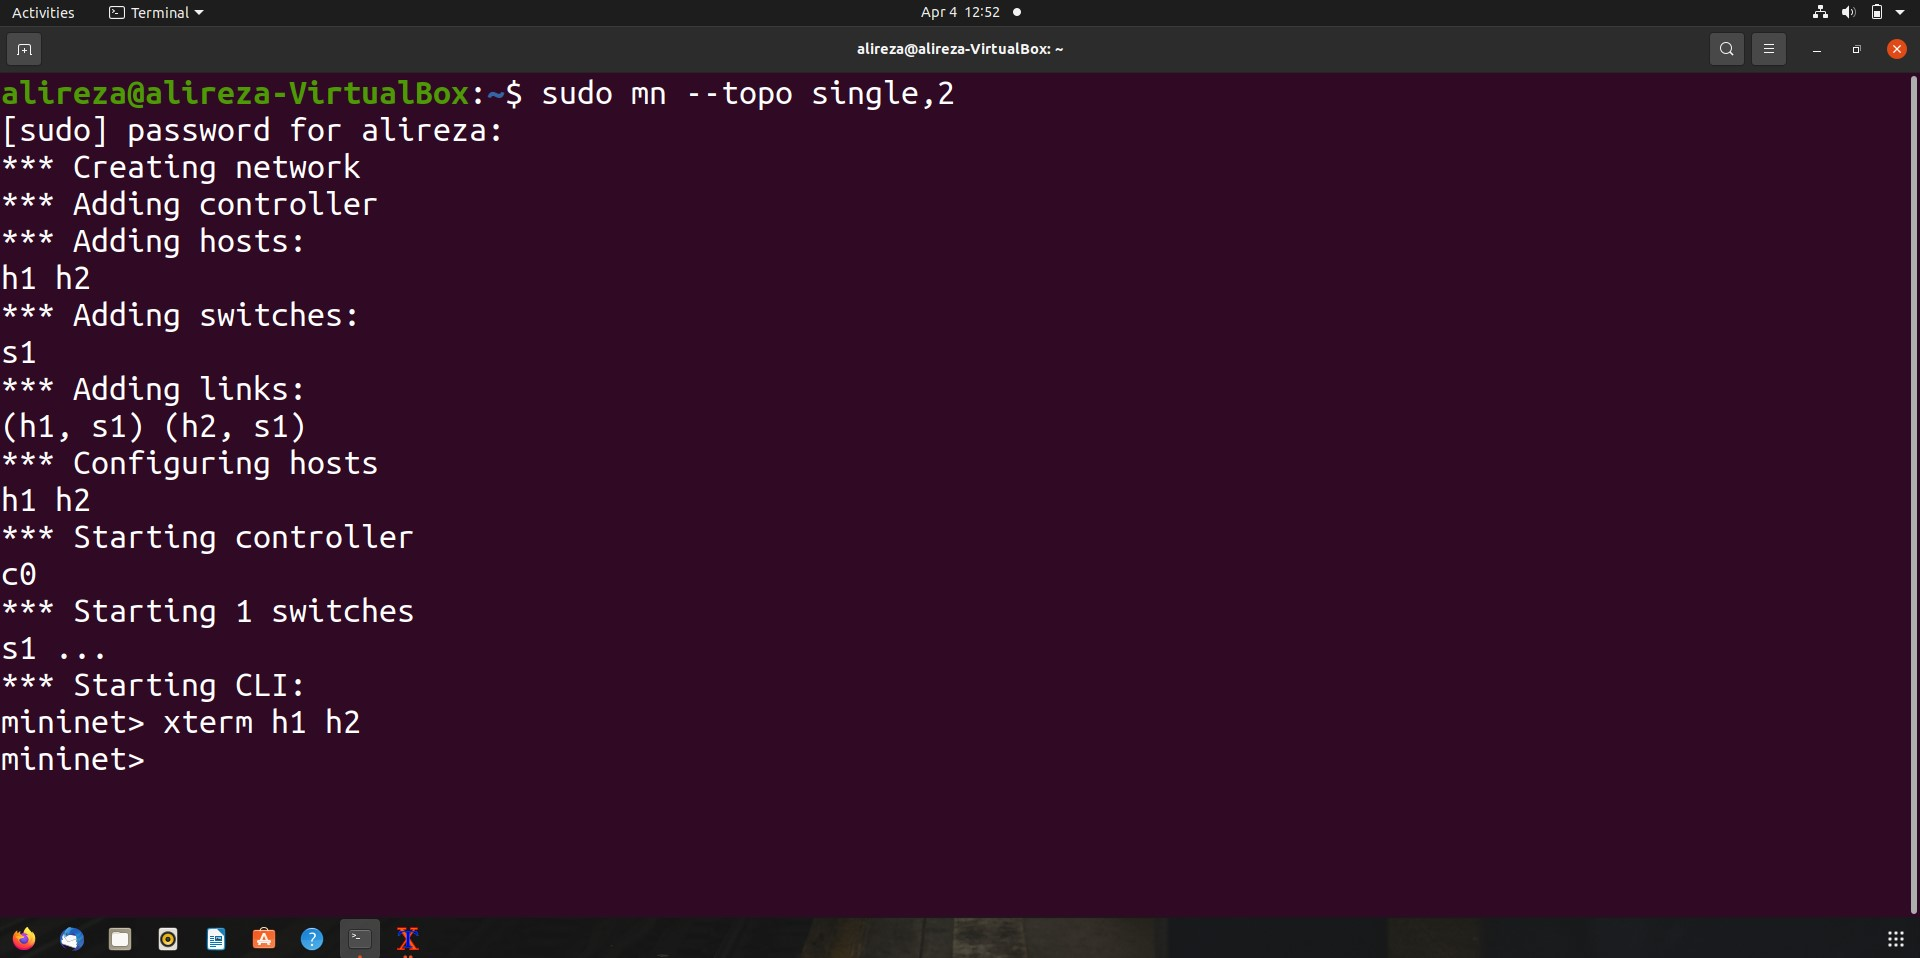
\includegraphics[width=1.0\textwidth]{figures/2a.jpg}
    \caption
	{
خروجی دستور \lr{sudo mn --topo single,3}
	}
    \label{fig:fig1}
\end{figure}

\subsection{دستور \lr{nodes}}
دستور \lr{nodes}، نودهای موجود در شبکه را نشان می‌دهد.
\begin{figure}[H]
    \centering
    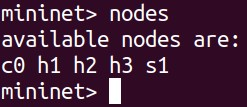
\includegraphics[width=0.3\textwidth]{figures/2b.jpg}
    \caption
	{
خروجی دستور \lr{nodes}
	}
    \label{fig:fig1}
\end{figure}
همانطور که می‌بینیم، دستور \lr{nodes}، همه‌ی نودهای حاضر در شبکه‌ی ساخته شده اعم از کنترلر، سوئیچ و میزبان را لیست می‌کند. در اینجا یک کنترلر (\lr{c0})، سه میزبان (\lr{h1}، \lr{h2}، \lr{h3}) و یک سوئیچ (\lr{s1}) در شبکه موجودند.

\subsection{دستور \lr{net}}
دستور \lr{net}، لینک‌های موجود بین دیوایس‌های \lr{Mininet} در شبکه را برای درک بهتر توپولوژی شبکه نشان می‌دهد.
\begin{figure}[H]
    \centering
    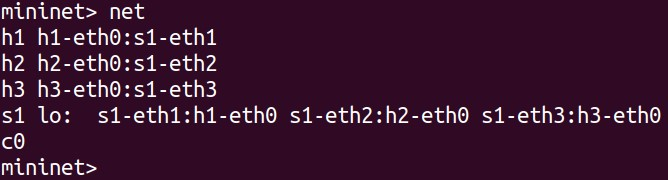
\includegraphics[width=0.5\textwidth]{figures/2c.jpg}
    \caption
	{
خروجی دستور \lr{net}
	}
    \label{fig:fig1}
\end{figure}
همانطور که می‌بینیم، دستور \lr{net}، همه‌ی لینک‌های موجود در شبکه را لیست می‌کند.
در اینجا به ترتیب اینترفیسِ \lr{eth0} از میزبانِ \lr{h1} به \lr{eth1} از سوئیچِ \lr{s1}، اینترفیسِ \lr{eth0} از میزبانِ \lr{h2} به \lr{eth2} از سوئیچِ \lr{s1}، اینترفیسِ \lr{eth0} از میزبانِ \lr{h3} به \lr{eth3} از سوئیچِ \lr{s1} وصل است.
سوئیچِ \lr{s1} دارای یک اینترفیسِ \lr{loopback} به نام \lr{lo} است.
سوئیچِ \lr{s1} به اینترفیسِ \lr{h1-eth0} از طریق اینترفیسِ \lr{s1-eth1} متصل است.
سوئیچِ \lr{s1} به اینترفیسِ \lr{h2-eth0} از طریق اینترفیسِ \lr{s1-eth2} متصل است.
سوئیچِ \lr{s1} به اینترفیسِ \lr{h3-eth0} از طریق اینترفیسِ \lr{s1-eth3} متصل است.
کنترلرِ \lr{c0} مغز شبکه است که یک دانش جامع از درباره‌ی شبکه دارد. یک کنترلر سوئیچ‌ها را در نحوه‌ی \lr{forward} یا \lr{drop} کردن بسته‌ها در شبکه راهنمایی می‌کند.

\subsection{دستور \lr{dump}}
دستور \lr{dump}، اطلاعات از قبیل نوع دیوایس، آدرس آی‌پی‌ها و شناسه پروسس‌های نودهای موجود در شبکه را نشان می‌دهد.
\begin{figure}[H]
    \centering
    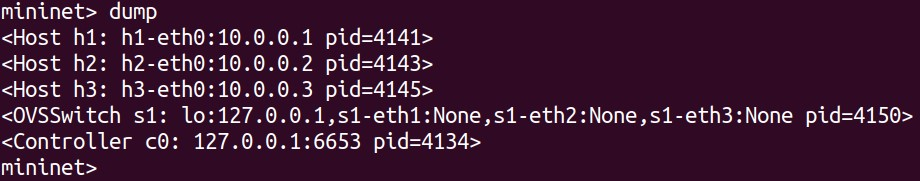
\includegraphics[width=0.75\textwidth]{figures/2d.jpg}
    \caption
	{
خروجی دستور \lr{dump}
	}
    \label{fig:fig1}
\end{figure}
همانطور که می‌بینیم، دستور \lr{dump}، اطلاعات دیوایس‌های موجود در شبکه را لیست می‌کند. در اینجا به ترتیب 
میزبانِ \lr{h1} دارای آدرس آی‌پیِ \lr{10.0.0.1} و پروسس آی‌دیِ 4141،
میزبانِ \lr{h2} دارای آدرس آی‌پیِ \lr{10.0.0.2} و پروسس آی‌دیِ 4143،
میزبانِ \lr{h3} دارای آدرس آی‌پیِ \lr{10.0.0.3} و پروسس آی‌دیِ 4145،
سوئیچِ \lr{s1} دارای آدرس آی‌پیِ لوپ‌بک \lr{127.0.0.1} و پروسس آی‌دیِ 4150،
کنترلرِ \lr{c0} دارای آدرس آی‌پیِ \lr{127.0.0.1} و پروسس آی‌دیِ 4134،

\section{}
\subsection{}
\subsubsection{\lr{Tree}}
توپولوژیِ \lr{Tree} که تحت عنوان \lr{star bus} نیز شناخته می‌شود، یک ساختار درخت‌گونه دارد که در آن همه‌ی کامپیوترها به یکدیگر همچون شاخه‌های درخت به درخت متصل شده‌اند. در شبکه‌های کامپیوتری، این توپولوژی ترکیبی از توپولوژی‌های \lr{Star} و \lr{Bus} است. مزیت اصلی این توپولوژی انعطاف‌پذیری (\lr{flexibility}) و مقیاس‌پذیری (\lr{Scalability}) است. این توپولوژی به عنوان ساده‌ترین توپولوژی در میان همه توپولوژی‌های دارای تنها یک روتر بین هر دو نود داخل شبکه است. الگوی اتصال شبیه درختی است که در آن همه شاخه ها از یک ریشه سرچشمه می گیرند و از این رو توپولوژی \lr{Tree} یکی از محبوب ترین توپولوژی‌ها در بین پنج توپولوژی شبکه است.
\newline
\newline
مزایا:

\begin{itemize}
\item [$\bullet$] این توپولوژی ترکیبی از توپولوژی \lr{Star} و \lr{Bus} است.
\item [$\bullet$] این توپولوژی چینش داده های سلسله مراتبی و مرکزی گره ها را فراهم می‌کند.
\item [$\bullet$] از آنجایی که نودهای برگ می‌توانند یک یا چند گره را در زنجیره سلسله مراتبی اضافه کنند، این توپولوژی مقیاس‌پذیری بالایی را فراهم می‌کند.
\item [$\bullet$] اگر یکی از نودهای آن‌ها آسیب ببیند یا کار نکند، نودهای دیگر در یک شبکه تحت تأثیر قرار نمی‌گیرند.
\item [$\bullet$] توپولوژی \lr{Tree} تعمیر و نگهداری آسان را فراهم می‌کند و به آسانی می‌توان عیب‌یابی را انجام داد.
\item [$\bullet$] توپولوژی قابل فراخوانی (نودهای برگ می‌توانند نودهای بیشتری را نگه دارند.)
\item [$\bullet$] توسط چندین وندورِ سخت‌افزار و نرم‌افزار پشتیبانی می‌شود.
\item [$\bullet$] سیم کشی نقطه‌به‌نقطه برای بخش‌های جداگانه.
\end{itemize}
معایب:
\begin{itemize}
\item [$\bullet$] پیکربندی این شبکه در مقایسه با سایر توپولوژی‌های شبکه بسیار دشوار است.
\item [$\bullet$] طول یک بخش محدود است و محدودیت سگمنت به نوع کابل‌کشی استفاده شده بستگی دارد.
\item [$\bullet$] به دلیل وجود تعداد زیادی نود، عملکرد شبکه توپولوژی \lr{Tree} کمی کند می‌شود.
\item [$\bullet$] اگر کامپیوتر سطح اول خطا داشته باشد، کامپیوتر سطح بعدی نیز دچار مشکل خواهد شد.
\item [$\bullet$] در مقایسه با توپولوژی \lr{Star} و \lr{Ring}، به تعداد زیادی کابل نیاز دارد.
\item [$\bullet$] از آنجایی که داده‌ها باید از کابل مرکزی منتقل شوند، ترافیک شبکه متراکمی ایجاد می‌کند.
\item [$\bullet$] \lr{Backbone} به عنوان نقطه شکست کل بخش شبکه ظاهر می‌شود.
\item [$\bullet$] تعمیر این توپولوژی بسیار پیچیده است.
\item [$\bullet$] هزینه تاسیسات نیز افزایش می‌یابد.
\item [$\bullet$] اگر بخش عمده‌ای از نودها در این شبکه اضافه شوند، تعمیر و نگهداری پیچیده خواهد شد.

\end{itemize}

\begin{figure}[H]
    \centering
    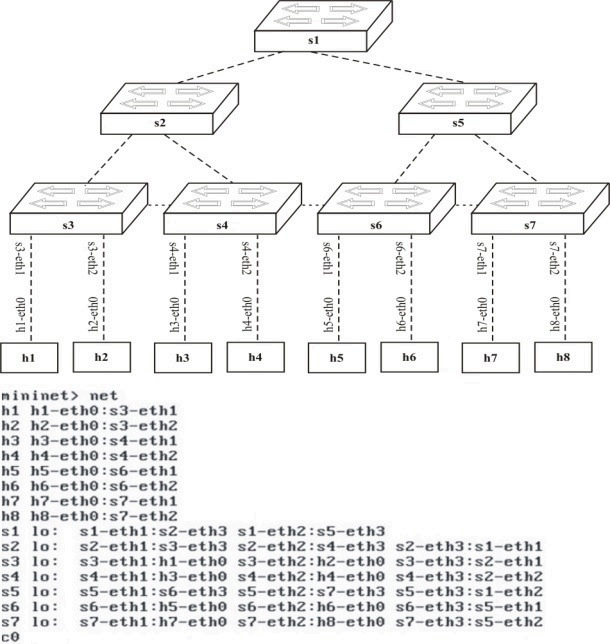
\includegraphics[width=0.5\textwidth]{figures/3a.jpg}
    \caption
	{
ساختار توپولوژیِ \lr{Tree} 
	}
    \label{fig:fig1}
\end{figure}
%%%%%%%%%%%%%
\subsubsection{\lr{Linear}}
توپولوژی \lr{Linear} از یک کابل اصلی با یک پایانه در هر انتها تشکیل شده است. تمام نودها (سرور فایل، ورک‌استیشن‌ها و تجهیزات جانبی) به کابل خطی متصل هستند. توپولوژی خطی شامل \lr{k} سوئیچ و \lr{k} میزبان است. همچنین یک پیوند بین هر سوئیچ و هر میزبان در میان سوئیچ‌ها ایجاد می‌کند. این توپولوژی در واقع نوعی توپولوژی شبکه است که در آن هر دستگاه یکی پس از دیگری در یک زنجیره متوالی به هم متصل می‌شود. در این حالت \lr{Bus} اتصال شبکه بین دستگاه‌ها است. اگر هر پیوندی در زنجیره شبکه قطع شود، تمام انتقال شبکه متوقف می‌شود. برای شبکه‌های کوچک کارآمد است. زیرا راه اندازی آن ساده است و از کابل‌های کوتاه‌تری استفاده می‌کند زیرا هر دستگاه به دستگاه بعدی متصل می‌شود. با این حال، این یک راه حل ضعیف برای شبکه‌های بزرگتر است، زیرا کل شبکه به هر اتصال متکی است و با اضافه شدن دستگاه‌های بیشتر، سرعت شبکه کاهش می‌یابد.
\newline
\newline
مزایا:

\begin{itemize}
\item [$\bullet$] اتصال کامپیوتر یا دستگاه جانبی به \lr{Bus} خطی آسان است.
\item [$\bullet$] نسبت به توپولوژی \lr{Star} به طول کابل کمتری نیاز دارد.
\end{itemize}
معایب:
\begin{itemize}
\item [$\bullet$] در صورت قطع شدن کابل اصلی، کل شبکه قطع می‌شود.
\item [$\bullet$] ترمیناتورها در هر دو انتهای کابل \lr{Backbone} مورد نیاز هستند.
\item [$\bullet$] اگر کل شبکه قطع شود، شناسایی مشکل دشوار است.
\item [$\bullet$] قرار نیست به عنوان یک راه حل مستقل در یک ساختمان بزرگ استفاده شود.

\end{itemize}

\begin{figure}[H]
    \centering
    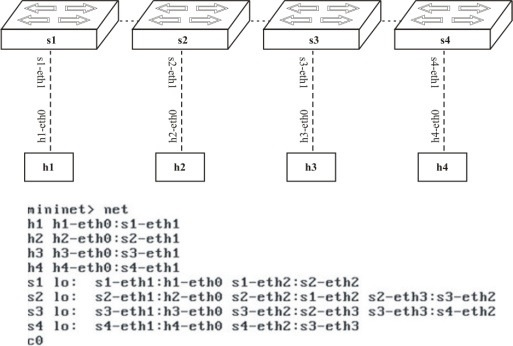
\includegraphics[width=0.5\textwidth]{figures/3b.jpg}
    \caption
	{
ساختار توپولوژیِ \lr{Linear} 
	}
    \label{fig:fig1}
\end{figure}
%%%%%%%%%%%%%
\subsubsection{\lr{Reversed}}
این یک توپولوژی ساده با یک سوئیچ \lr{Openflow} و \lr{k} میزبان است. همچنین یک پیوند بین سوئیچ و \lr{k} میزبان ایجاد می‌کند. در واقع این توپولوژی همان توپولوژیِ \lr{Single} است و فقط ترتیب اتصال اینترفیس‌ها برعکس است. در توپولوژی‌های ستاره‌ای (\lr{Single}  و \lr{Reversed}) همه دستگاه‌ها از طریق یک کابل به یک سوئیچ واحد متصل می‌شوند. این سوئیچ نود مرکزی است و تمام نودهای دیگر به نود مرکزی متصل هستند.
\newline
\newline
مزایا:

\begin{itemize}
\item [$\bullet$] اگر \lr{n}  دستگاه در این توپولوژی  به یکدیگر متصل شده باشند، تعداد کابل های مورد نیاز برای اتصال آنها \lr{n}  است. بنابراین، تنظیم آن آسان است.
\item [$\bullet$] هر دستگاه برای اتصال به سوئیچ فقط به 1 پورت نیاز دارد، بنابراین تعداد کل پورت‌های مورد نیاز \lr{n} است.
\end{itemize}
معایب:
\begin{itemize}
\item [$\bullet$] اگر سوئیچ که کل توپولوژی به آن متکی است از کار بیفتد، کل سیستم از کار می‌افتد.
\item [$\bullet$] هزینه نصب بالاست.
\item [$\bullet$] عملکرد بر اساس متمرکز کننده منفرد یعنی سوئیچ است.

\end{itemize}


\begin{figure}[H]
    \centering
    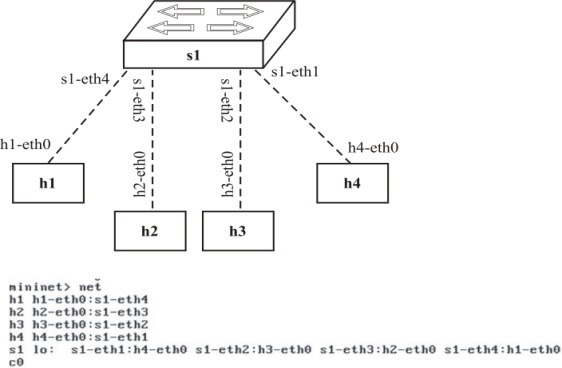
\includegraphics[width=0.5\textwidth]{figures/3c.jpg}
    \caption
	{
ساختار توپولوژیِ \lr{Reversed} 
	}
    \label{fig:fig1}
\end{figure}


\subsection{}
\subsubsection{\lr{Tree}}
برای ساخت شبکه‌ای با توپولوژیِ \lr{Tree} با عمقِ 3 (8 میزبان) دستور زیر را اجرا می‌کنیم.
\begin{latin}
\$ sudo mn --topo tree,depth=3
\end{latin}
\begin{figure}[H]
    \centering
    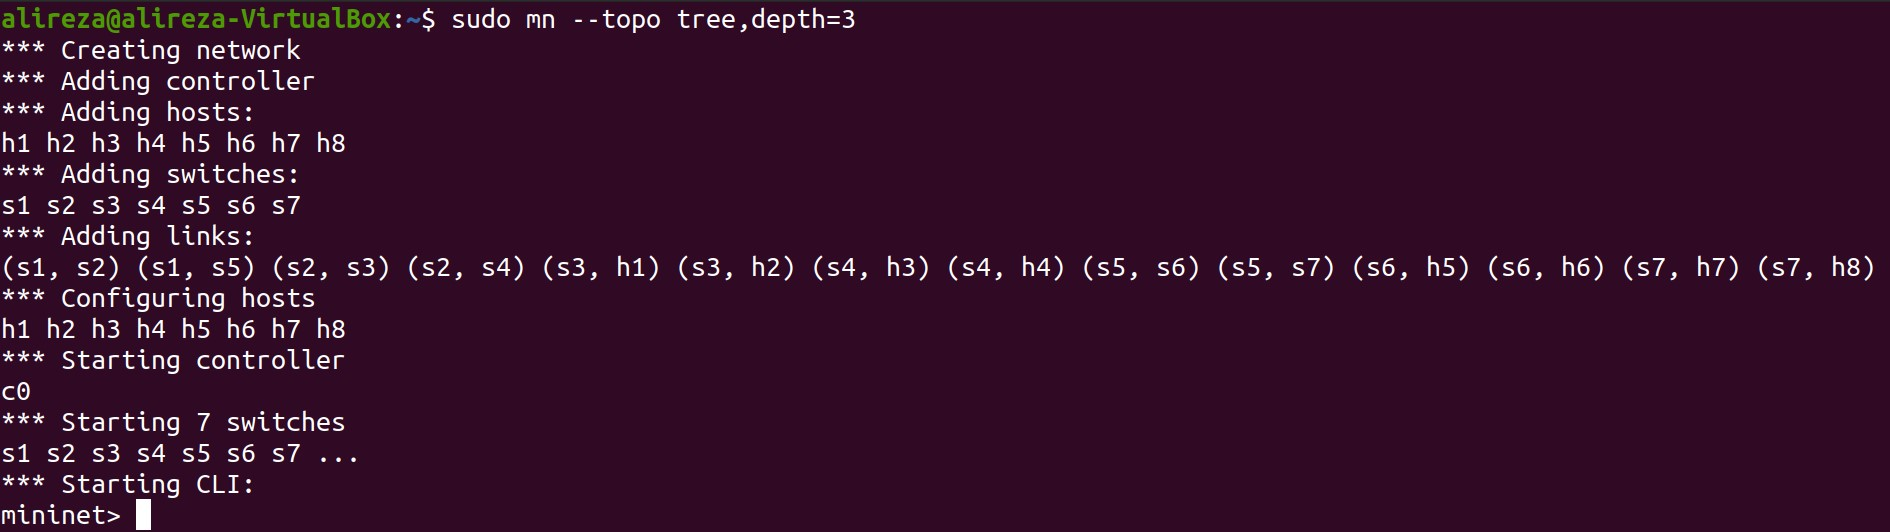
\includegraphics[width=1.0\textwidth]{figures/3d.jpg}
    \caption
	{
خروجی دستورِ \lr{sudo mn --topo tree,depth=3}
	}
    \label{fig:fig1}
\end{figure}
\begin{figure}[H]
    \centering
    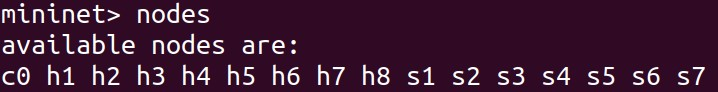
\includegraphics[width=0.7\textwidth]{figures/3d1.jpg}
    \caption
	{
\lr{nodes}
	}
    \label{fig:fig1}
\end{figure}
\begin{figure}[H]
    \centering
    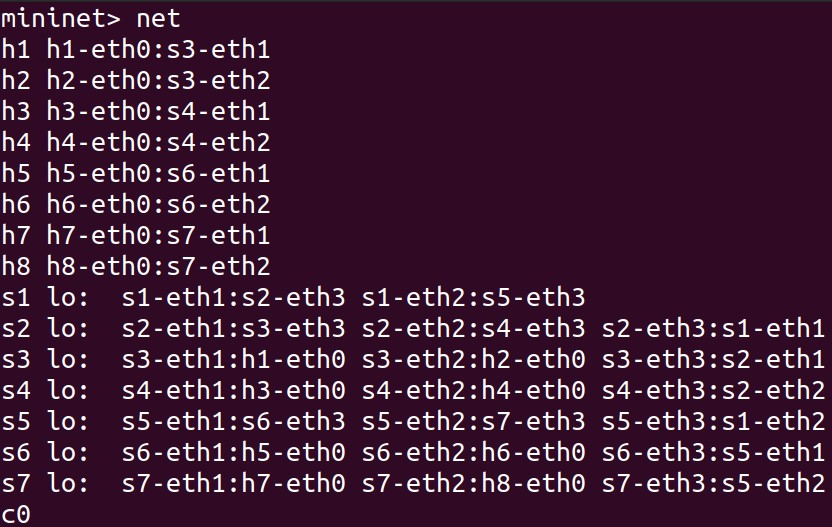
\includegraphics[width=0.7\textwidth]{figures/3d2.jpg}
    \caption
	{
\lr{net}
	}
    \label{fig:fig1}
\end{figure}
\begin{figure}[H]
    \centering
    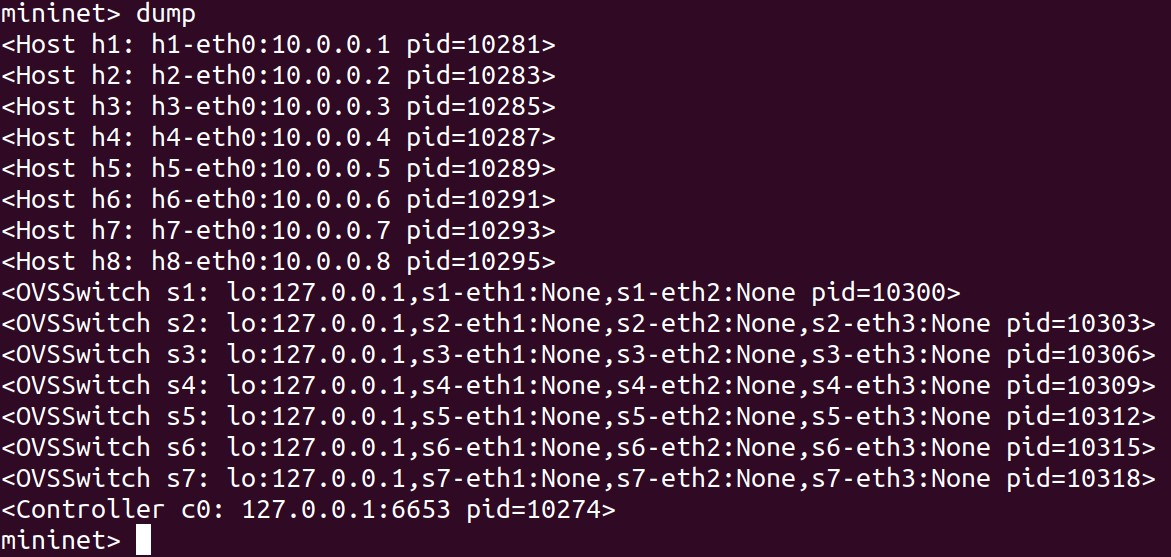
\includegraphics[width=1.0\textwidth]{figures/3d3.jpg}
    \caption
	{
\lr{dump}
	}
    \label{fig:fig1}
\end{figure}
%%%%%%%%%%%
\subsubsection{\lr{Linear}}
برای ساخت شبکه‌ای با توپولوژیِ \lr{Linear} با 1 کنترلر، 4 میزبان و 4 سوئیچ دستور زیر را اجرا می‌کنیم.
\begin{latin}
\$ sudo mn --topo linear,4
\end{latin}
\begin{figure}[H]
    \centering
    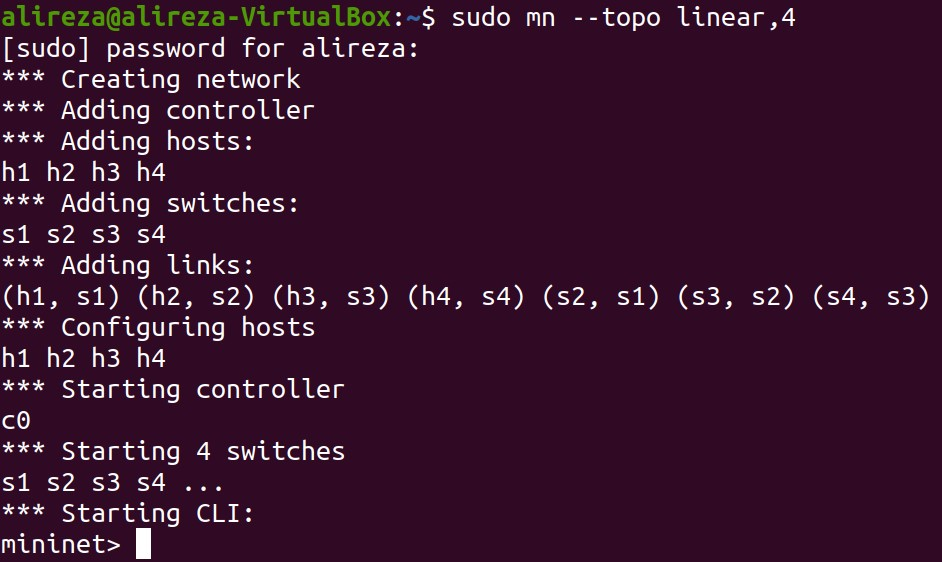
\includegraphics[width=1.0\textwidth]{figures/3e.jpg}
    \caption
	{
خروجی دستورِ \lr{sudo mn --topo linear,4}
	}
    \label{fig:fig1}
\end{figure}
\begin{figure}[H]
    \centering
    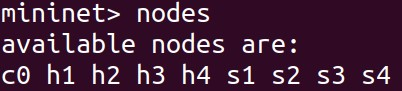
\includegraphics[width=0.7\textwidth]{figures/3e1.jpg}
    \caption
	{
\lr{nodes}
	}
    \label{fig:fig1}
\end{figure}
\begin{figure}[H]
    \centering
    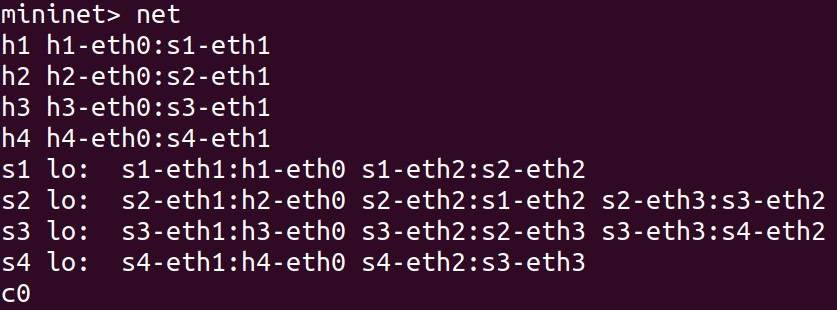
\includegraphics[width=0.7\textwidth]{figures/3e2.jpg}
    \caption
	{
\lr{net}
	}
    \label{fig:fig1}
\end{figure}
\begin{figure}[H]
    \centering
    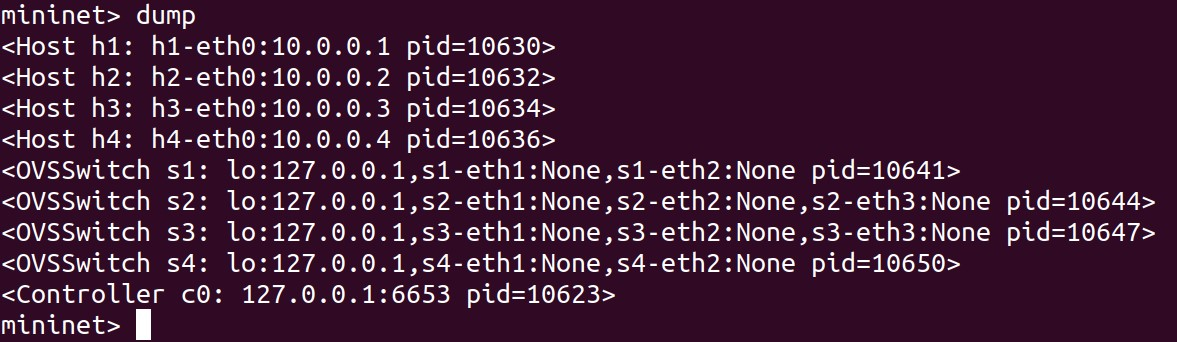
\includegraphics[width=1.0\textwidth]{figures/3e3.jpg}
    \caption
	{
\lr{dump}
	}
    \label{fig:fig1}
\end{figure}
%%%%%%%%%%%
\subsubsection{\lr{Reversed}}
برای ساخت شبکه‌ای با توپولوژیِ \lr{Reveresed} با 1 کنترلر، 4 میزبان و 4 سوئیچ دستور زیر را اجرا می‌کنیم.
\begin{latin}
\$ sudo mn --topo reversed,3
\end{latin}
\begin{figure}[H]
    \centering
    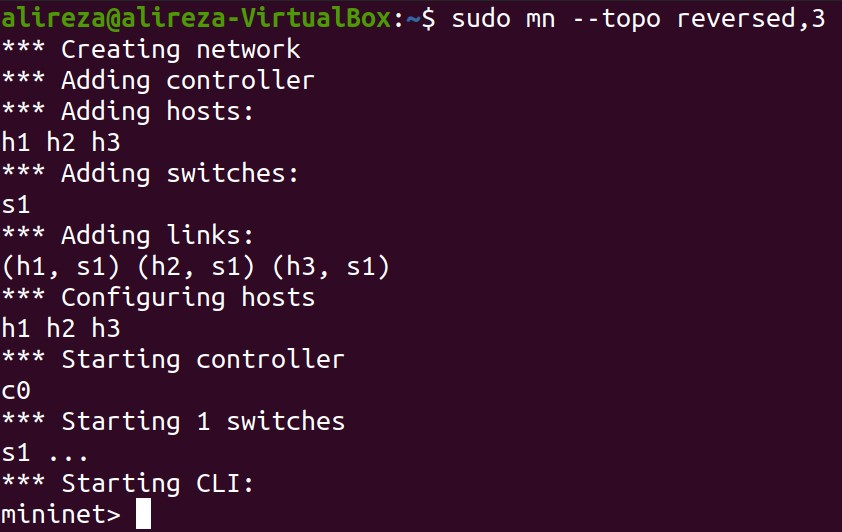
\includegraphics[width=1.0\textwidth]{figures/3f.jpg}
    \caption
	{
خروجی دستورِ \lr{sudo mn --topo reversed,3}
	}
    \label{fig:fig1}
\end{figure}
\begin{figure}[H]
    \centering
    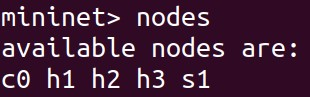
\includegraphics[width=0.7\textwidth]{figures/3f1.jpg}
    \caption
	{
\lr{nodes}
	}
    \label{fig:fig1}
\end{figure}
\begin{figure}[H]
    \centering
    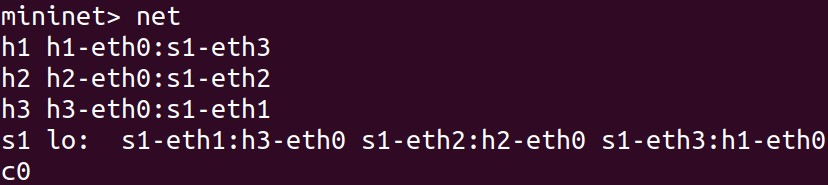
\includegraphics[width=0.7\textwidth]{figures/3f2.jpg}
    \caption
	{
\lr{net}
	}
    \label{fig:fig1}
\end{figure}
\begin{figure}[H]
    \centering
    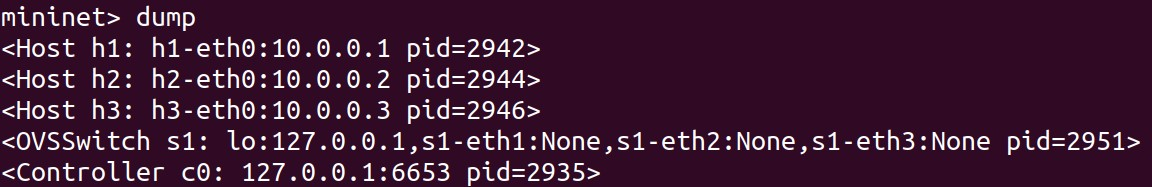
\includegraphics[width=1.0\textwidth]{figures/3f3.jpg}
    \caption
	{
\lr{dump}
	}
    \label{fig:fig1}
\end{figure}
%%%%%%%%%%%%%%%%%%%%%%%%%%%%%%%%%%%
%%%%%%%%%%%%%%%%%%%%%%%%%%%%%%%%%%%
%%%%%%%%%%%%%%%%%%%%%%%%%%%%%%%%%%%

\section*{منابع}
\renewcommand{\section}[2]{}%
\begin{thebibliography}{99} % assumes less than 100 references
%چنانچه مرجع فارسی نیز داشته باشید باید دستور فوق را فعال کنید و مراجع فارسی خود را بعد از این دستور وارد کنید


\begin{LTRitems}

\resetlatinfont

\bibitem{b1} http://mininet.org/overview/
\bibitem{b1} https://www.geeksforgeeks.org/advantages-and-disadvantages-of-tree-topology/
\bibitem{b1} https://www.guru99.com/type-of-network-topology.html
\bibitem{b1} https://slsdn.blogspot.com/2020/05/topologies-in-mininet.html
\bibitem{b1} https://fcit.usf.edu/network/chap5/chap5.htm
\end{LTRitems}

\end{thebibliography}


\end{document}
